% !TEX root = ../main.tex

% Exercises section

\section{Description and Visualization of Datasets}\label{appendix:sequences}
See below for the visualization of the five sequences whose change points are to be detected using MCMC-based Bayesian change point detection methods. The blue dots are the observed values and the orange lines show the underlying means of each segment. The number of observation ($n$), number of change points ($k$), true segment means ($\bm{\mu}$), true change point locations ($\bm{r}$), and the number of possible configurations of change points ($T$) are shown in the plots below. Note that the $x$-axis indicate the index or order in time, and the $y$-axis are the values of the observations.
\begin{figure}[H]
    \centering
    \begin{subfigure}{.3\textwidth}
    	\centering
        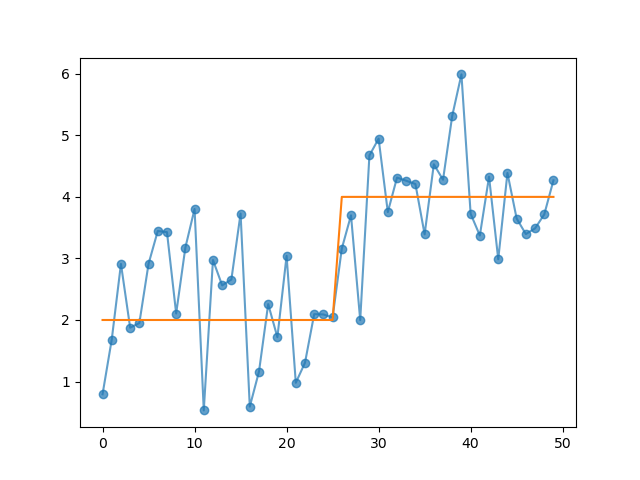
\includegraphics[width=\linewidth]{../../plots/sequence_M2_N50_seed1_diffind2.png}
        \caption{$n=50, k=1, \bm{\mu} = \{2, 4\}, \bm{r} = \{25\}, T = 49$}
    \end{subfigure}
    \begin{subfigure}{.3\textwidth}
        \centering
    	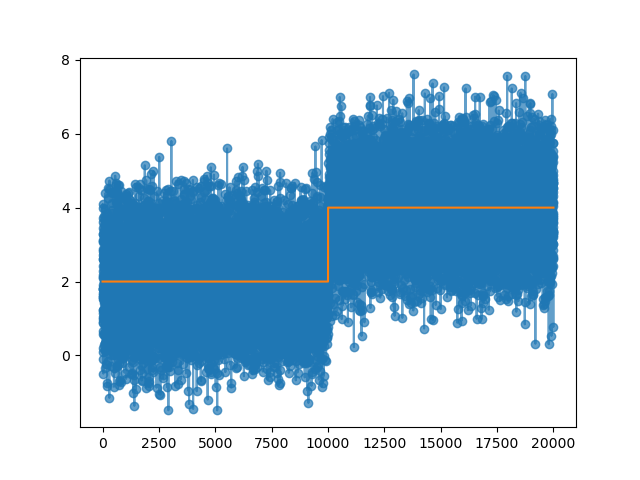
\includegraphics[width=\linewidth]{../../plots/sequence_M2_N20000_seed1_diffind2.png}
    	\caption{$n=20000, k=1, \bm{\mu} = \{2, 4\}, \bm{r} = \{10000\}, T = 19999$}
	\end{subfigure}
	\begin{subfigure}{.3\textwidth}
	    \centering
    	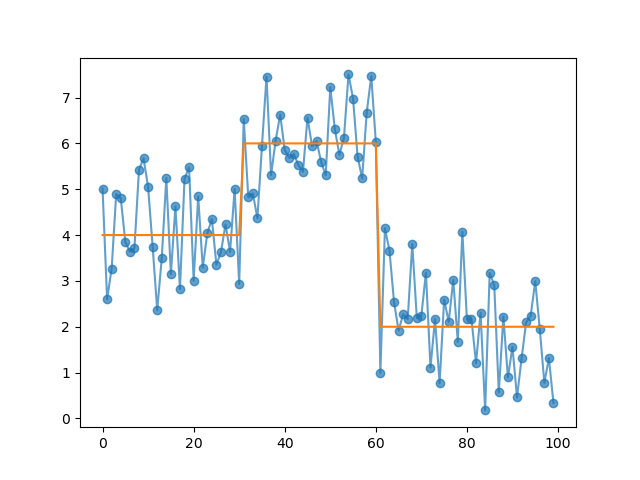
\includegraphics[width=\linewidth]{../../plots/sequence_M3_N100_seed2_diffind2.png}
    	\caption{$n=100, k=2, \bm{\mu} = \{4, 6, 2\}, \bm{r} = \{30, 60\}, T = 4851$}
	\end{subfigure}
	\begin{subfigure}{.3\textwidth}
	    \centering
    	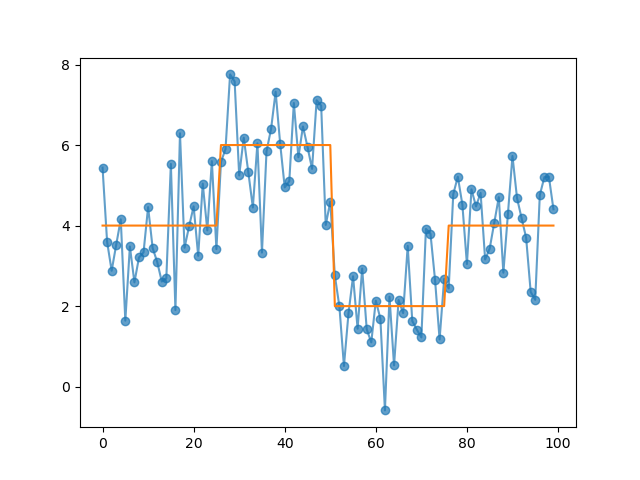
\includegraphics[width=\linewidth]{../../plots/sequence_M4_N100_seed3_diffind2.png}
    	\caption{$n=100, k=3, \bm{\mu} = \{4, 6, 2,4\}, \bm{r} = \{25, 50, 75\}, T = 156849$}
	\end{subfigure}
	\begin{subfigure}{.3\textwidth}
	    \centering
    	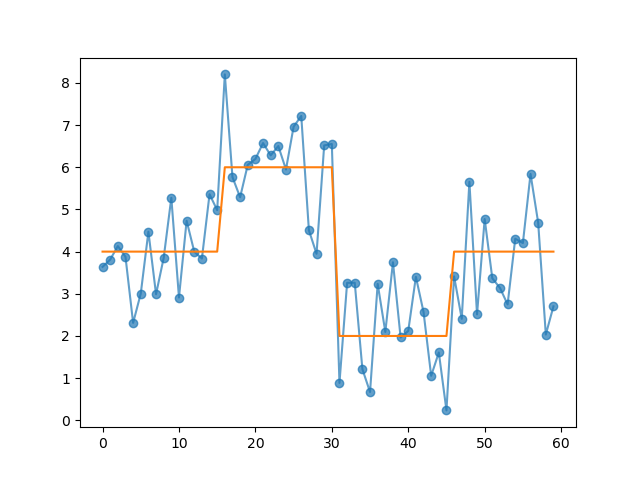
\includegraphics[width=\linewidth]{../../plots/sequence_M4_N60_seed3_diffind2.png}
    	\caption{$n=60, k=3, \bm{\mu} = \{4, 6, 2,4\}, \bm{r} = \{15, 30, 45\}, T = 32509$}
	\end{subfigure}
	\label{fig:sequences_viz}
	\caption{Visualization of sequences with change points to be detected.}
\end{figure}

\section{Sample Size Comparison}\label{appendix:sample}
See below for a comparison of the size of the samples generated by each MCMC sampler for each of the five sequences. For each model, the medians (solid lines), the $25$th and the $75$th percentiles (dashed lines) of the number of samples generated by each MCMC sampler are plotted across the amount of time elapsed since the start of the simulation. Note that in this particular plot, for each sequence, the samples of each MCMC sampler is trimmed to the minimum sample sizes across all five runs.
\begin{figure}[H]
    \centering
    \begin{subfigure}{.3\textwidth}
    	\centering
        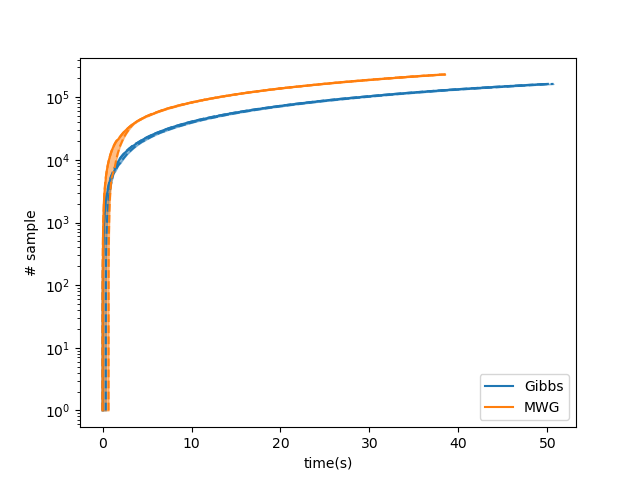
\includegraphics[width=\linewidth]{../../plots/SampleTime_M2_N50_NMCMC1_seed0_diffind2.png}
        \caption{$n=50, k=1$}
    \end{subfigure}
    \begin{subfigure}{.3\textwidth}
        \centering
    	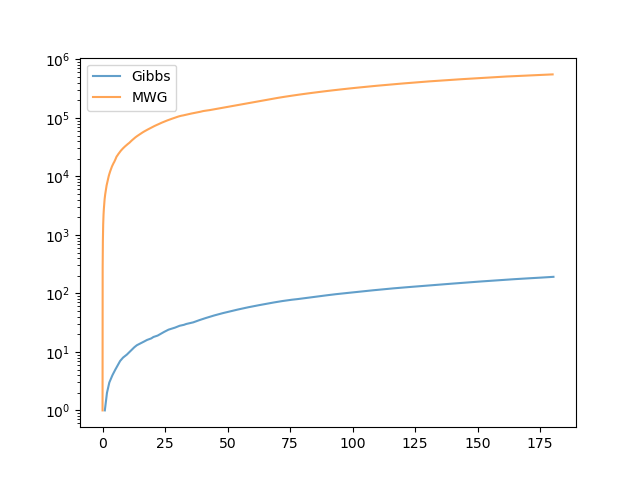
\includegraphics[width=\linewidth]{../../plots/SampleTime_M2_N20000_NMCMC3_seed0_diffind2.png}
    	\caption{$n=20000, k=1$}
	\end{subfigure}
	\begin{subfigure}{.3\textwidth}
	    \centering
    	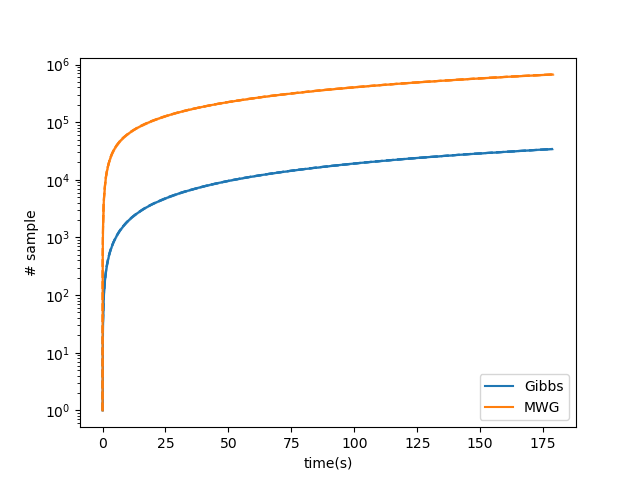
\includegraphics[width=\linewidth]{../../plots/SampleTime_M3_N100_NMCMC3_seed0_diffind2.png}
    	\caption{$n=100, k=2$}
	\end{subfigure}
	\begin{subfigure}{.3\textwidth}
	    \centering
    	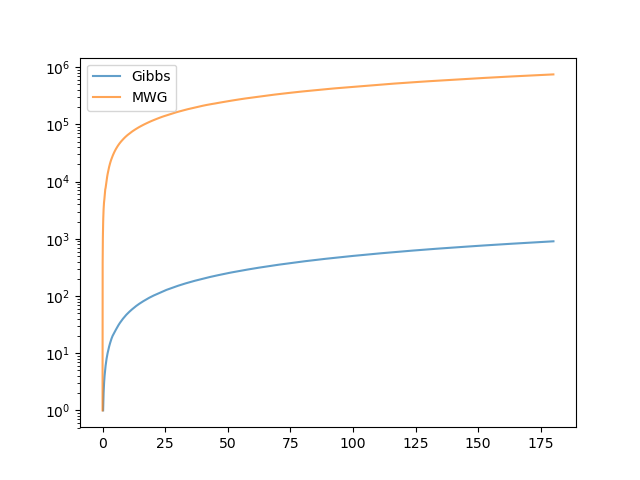
\includegraphics[width=\linewidth]{../../plots/SampleTime_M4_N100_NMCMC3_seed0_diffind2.png}
    	\caption{$n=100, k=3$}
	\end{subfigure}
	\begin{subfigure}{.3\textwidth}
	    \centering
    	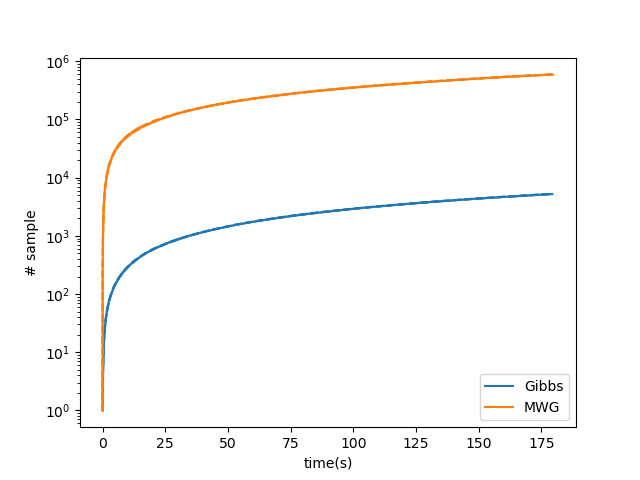
\includegraphics[width=\linewidth]{../../plots/SampleTime_M4_N60_NMCMC3_seed0_diffind2.png}
    	\caption{$n=60, k=3$}
	\end{subfigure}
	\caption{Number of samples generated by each MCMC sampler for each of the five sequences.}
\end{figure}

\section{Trace plots of entire sequences}\label{appendix:trace_full}

Each of the five figures below show the trace plots of the change points across the five runs for each sequence. Note that the trace plots include all samples generated by both MCMC samplers. Each color represents a distinct change point. For each plot, the $x$-axis indicate the number of the sample, and the $y$-axis represent the values of each sample (locations of change points).

\begin{figure}[H]
    \centering
    \begin{subfigure}{.3\textwidth}
    	\centering
        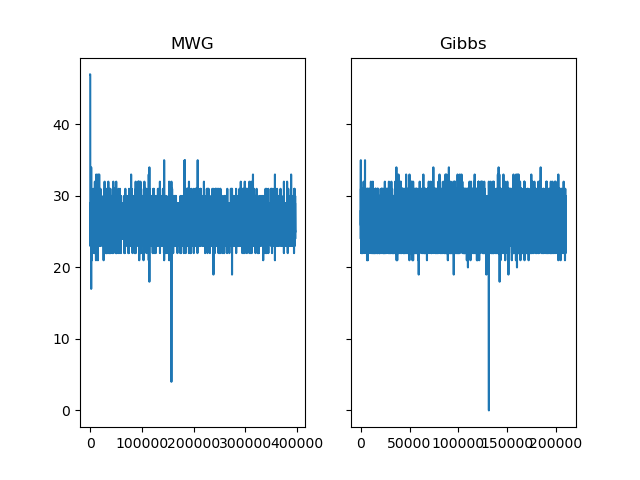
\includegraphics[width=\linewidth]{../../plots/Trace_M2_N50_NMCMC1_seed0_diffind2.png}
        \caption{simulation run \#1}
    \end{subfigure}
    \begin{subfigure}{.3\textwidth}
        \centering
    	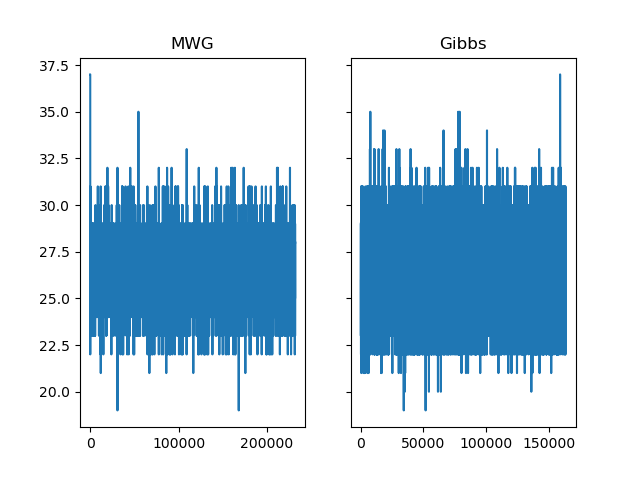
\includegraphics[width=\linewidth]{../../plots/Trace_M2_N50_NMCMC1_seed1_diffind2.png}
    	\caption{simulation run \#2}
	\end{subfigure}
	\begin{subfigure}{.3\textwidth}
	    \centering
    	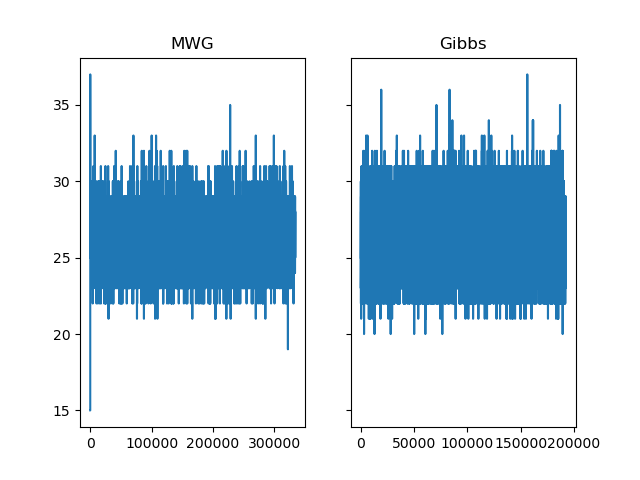
\includegraphics[width=\linewidth]{../../plots/Trace_M2_N50_NMCMC1_seed2_diffind2.png}
    	\caption{simulation run \#3}
	\end{subfigure}
	\begin{subfigure}{.3\textwidth}
	    \centering
    	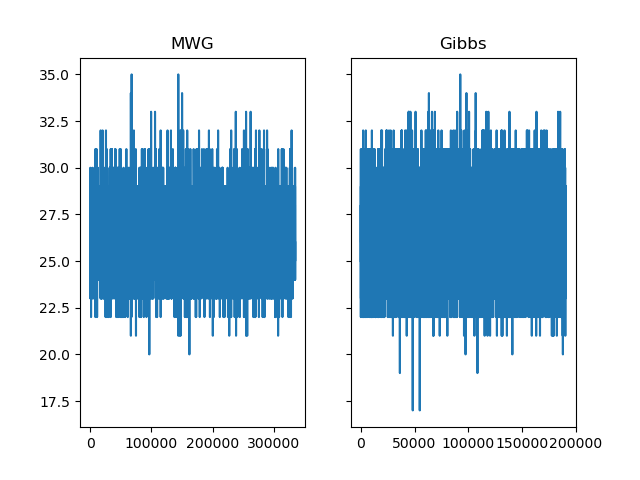
\includegraphics[width=\linewidth]{../../plots/Trace_M2_N50_NMCMC1_seed3_diffind2.png}
    	\caption{simulation run \#4}
	\end{subfigure}
	\begin{subfigure}{.3\textwidth}
	    \centering
    	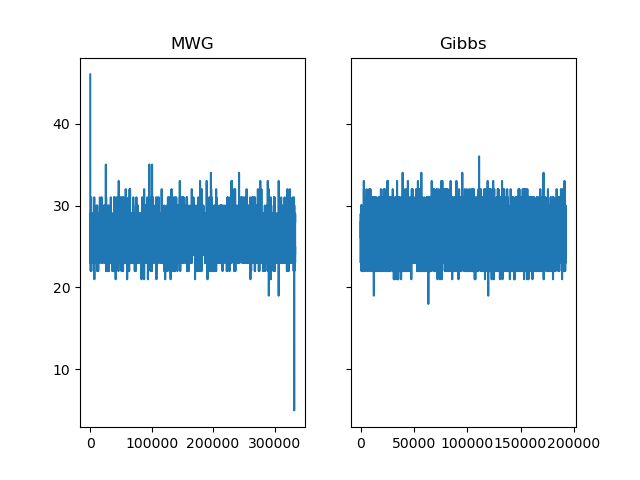
\includegraphics[width=\linewidth]{../../plots/Trace_M2_N50_NMCMC1_seed4_diffind2.png}
    	\caption{simulation run \#5}
	\end{subfigure}
	\caption{Trace plots of entire simulations for the sequence with $n=50, k=1, \bm{\mu} = \{2,4\}, \bm{r} = \{25\}, T=49$.}
\end{figure}

\begin{figure}[H]
    \centering
    \begin{subfigure}{.3\textwidth}
    	\centering
        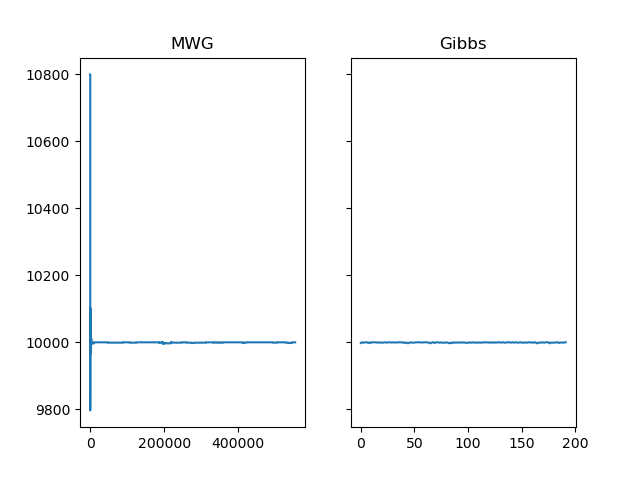
\includegraphics[width=\linewidth]{../../plots/Trace_M2_N20000_NMCMC3_seed0_diffind2.png}
        \caption{simulation run \#1}
    \end{subfigure}
    \begin{subfigure}{.3\textwidth}
        \centering
    	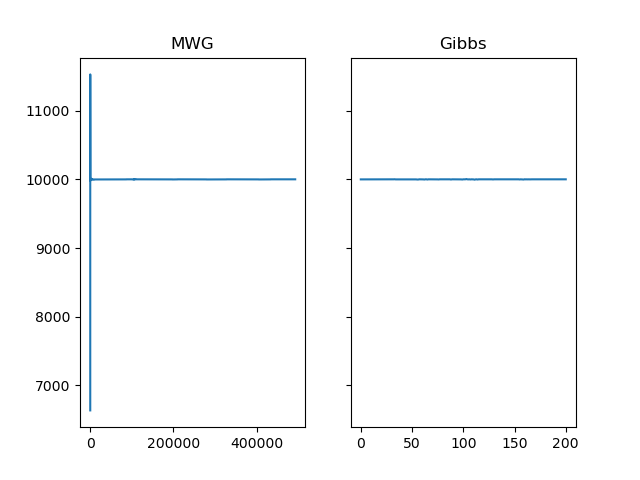
\includegraphics[width=\linewidth]{../../plots/Trace_M2_N20000_NMCMC3_seed1_diffind2.png}
    	\caption{simulation run \#2}
	\end{subfigure}
	\begin{subfigure}{.3\textwidth}
	    \centering
    	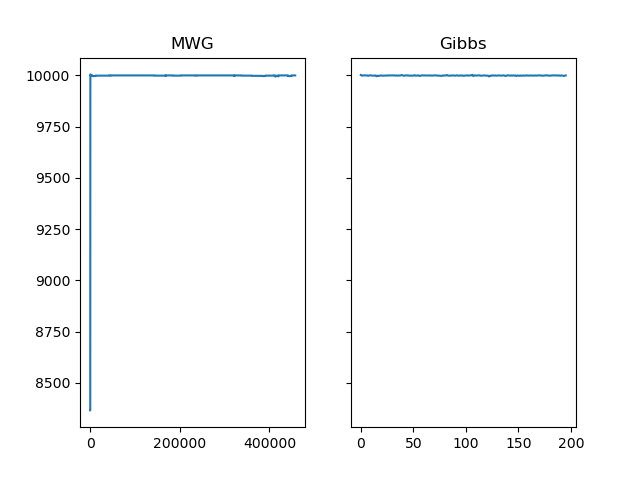
\includegraphics[width=\linewidth]{../../plots/Trace_M2_N20000_NMCMC3_seed2_diffind2.png}
    	\caption{simulation run \#3}
	\end{subfigure}
	\begin{subfigure}{.3\textwidth}
	    \centering
    	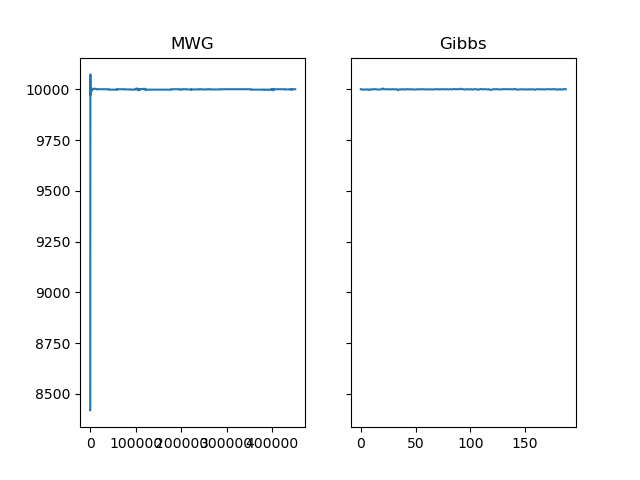
\includegraphics[width=\linewidth]{../../plots/Trace_M2_N20000_NMCMC3_seed3_diffind2.png}
    	\caption{simulation run \#4}
	\end{subfigure}
	\begin{subfigure}{.3\textwidth}
	    \centering
    	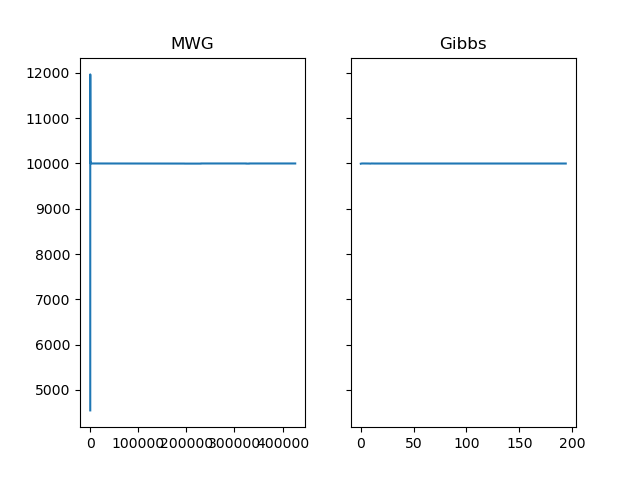
\includegraphics[width=\linewidth]{../../plots/Trace_M2_N20000_NMCMC3_seed4_diffind2.png}
    	\caption{simulation run \#5}
	\end{subfigure}
	\caption{Trace plots of entire simulations for the sequence with $n=20000, k=1, \bm{\mu} = \{2,4\}, \bm{r} = \{10000\}, T=19999$.}
\end{figure}

\begin{figure}[H]
    \centering
    \begin{subfigure}{.3\textwidth}
    	\centering
        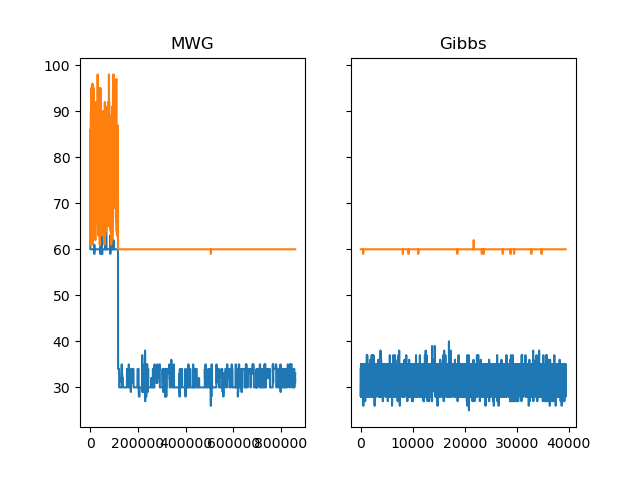
\includegraphics[width=\linewidth]{../../plots/Trace_M3_N100_NMCMC3_seed0_diffind2.png}
        \caption{simulation run \#1}
    \end{subfigure}
    \begin{subfigure}{.3\textwidth}
        \centering
    	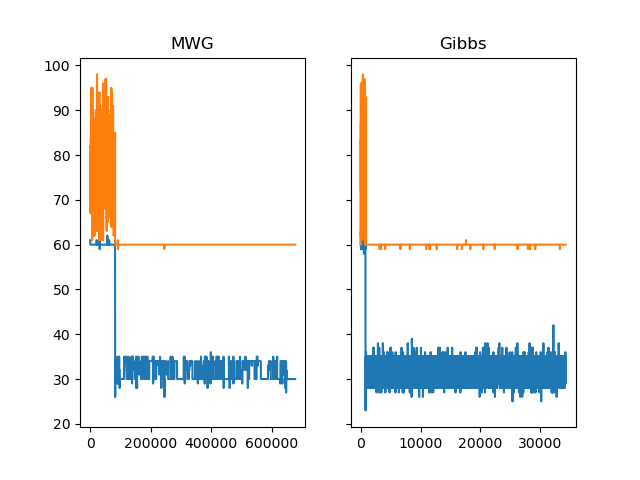
\includegraphics[width=\linewidth]{../../plots/Trace_M3_N100_NMCMC3_seed1_diffind2.png}
    	\caption{simulation run \#2}
	\end{subfigure}
	\begin{subfigure}{.3\textwidth}
	    \centering
    	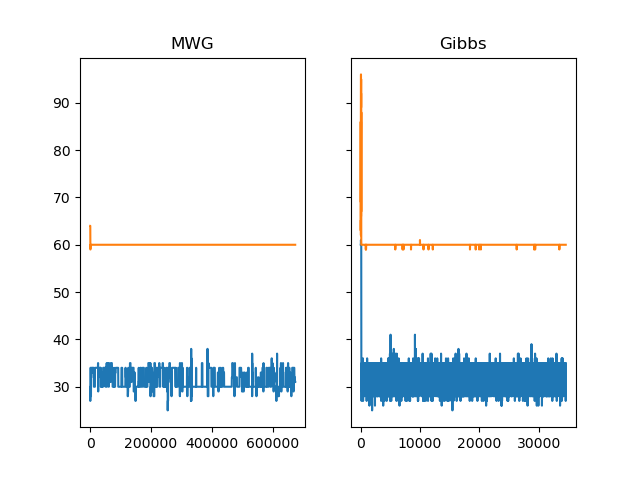
\includegraphics[width=\linewidth]{../../plots/Trace_M3_N100_NMCMC3_seed2_diffind2.png}
    	\caption{simulation run \#3}
	\end{subfigure}
	\begin{subfigure}{.3\textwidth}
	    \centering
    	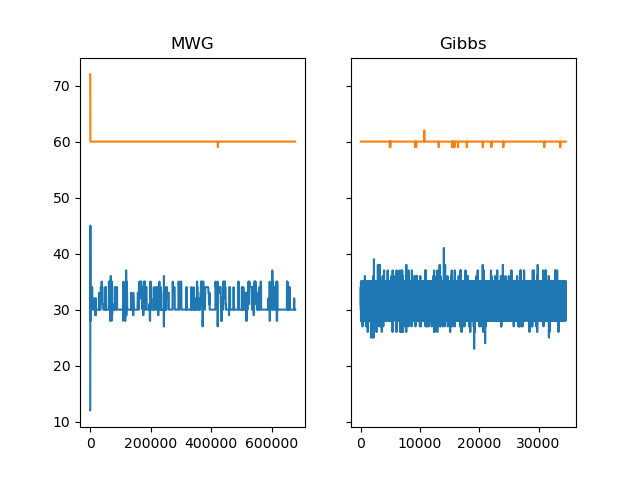
\includegraphics[width=\linewidth]{../../plots/Trace_M3_N100_NMCMC3_seed3_diffind2.png}
    	\caption{simulation run \#4}
	\end{subfigure}
	\begin{subfigure}{.3\textwidth}
	    \centering
    	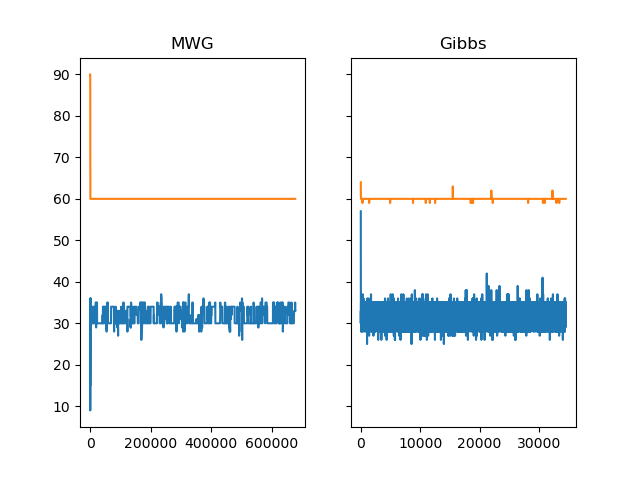
\includegraphics[width=\linewidth]{../../plots/Trace_M3_N100_NMCMC3_seed4_diffind2.png}
    	\caption{simulation run \#5}
	\end{subfigure}
	\caption{Trace plots of entire simulations for the sequence with $n=100, k=2, \bm{\mu} = \{4,6,2\}, \bm{r} = \{30, 60\}, T=4851$.}
\end{figure}

\begin{figure}[H]
    \centering
    \begin{subfigure}{.3\textwidth}
    	\centering
        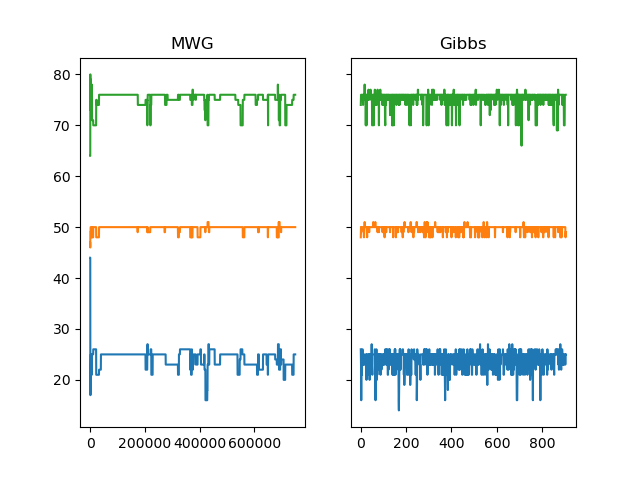
\includegraphics[width=\linewidth]{../../plots/Trace_M4_N100_NMCMC3_seed0_diffind2.png}
        \caption{simulation run \#1}
    \end{subfigure}
    \begin{subfigure}{.3\textwidth}
        \centering
    	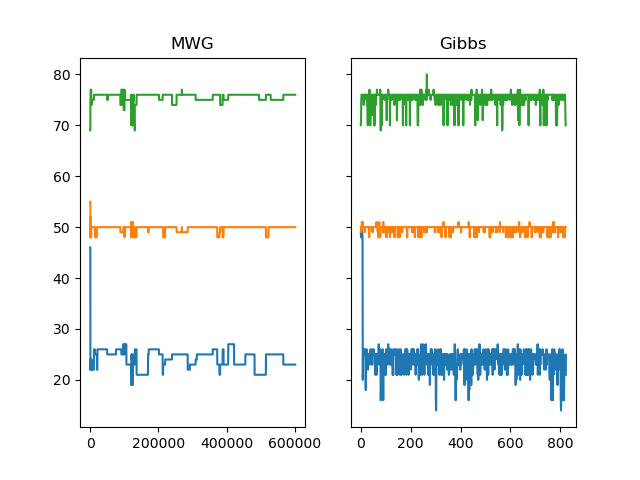
\includegraphics[width=\linewidth]{../../plots/Trace_M4_N100_NMCMC3_seed1_diffind2.png}
    	\caption{simulation run \#2}
	\end{subfigure}
	\begin{subfigure}{.3\textwidth}
	    \centering
    	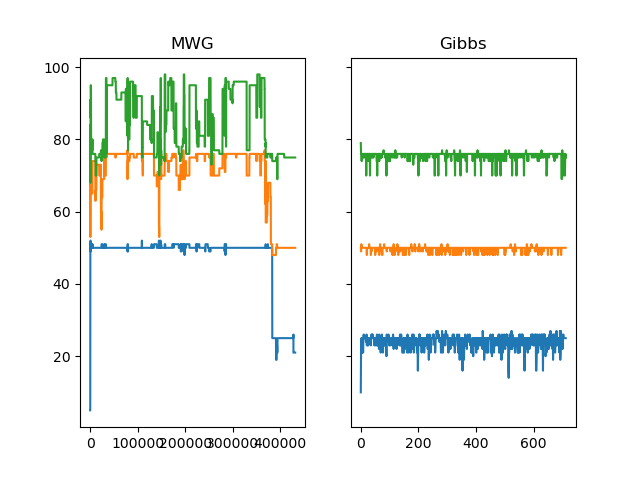
\includegraphics[width=\linewidth]{../../plots/Trace_M4_N100_NMCMC3_seed2_diffind2.png}
    	\caption{simulation run \#3}
	\end{subfigure}
	\begin{subfigure}{.3\textwidth}
	    \centering
    	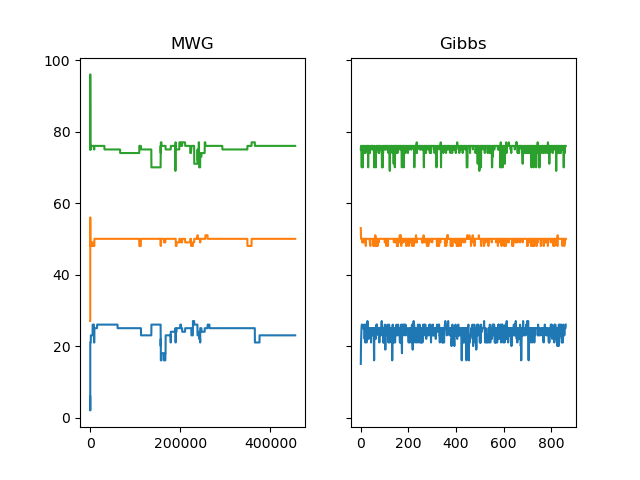
\includegraphics[width=\linewidth]{../../plots/Trace_M4_N100_NMCMC3_seed3_diffind2.png}
    	\caption{simulation run \#4}
	\end{subfigure}
	\begin{subfigure}{.3\textwidth}
	    \centering
    	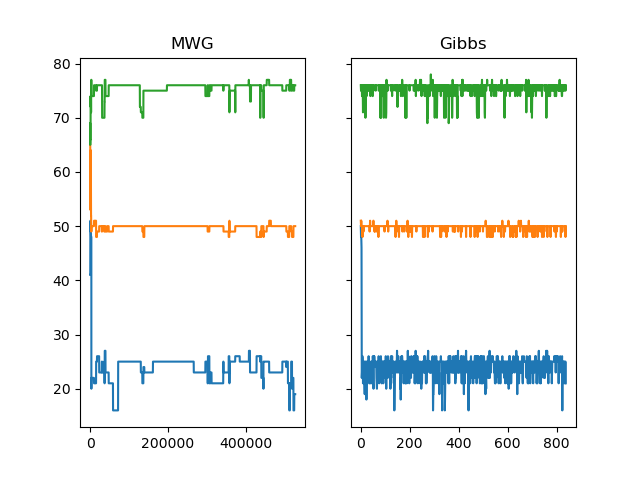
\includegraphics[width=\linewidth]{../../plots/Trace_M4_N100_NMCMC3_seed4_diffind2.png}
    	\caption{simulation run \#5}
	\end{subfigure}
	\caption{Trace plots of entire simulations for the sequence with $n=100, k=3, \bm{\mu} = \{4, 6, 2,4\}, \bm{r} = \{25, 50, 75\}, T = 156849$.}
\end{figure}

\begin{figure}[H]
    \centering
    \begin{subfigure}{.3\textwidth}
    	\centering
        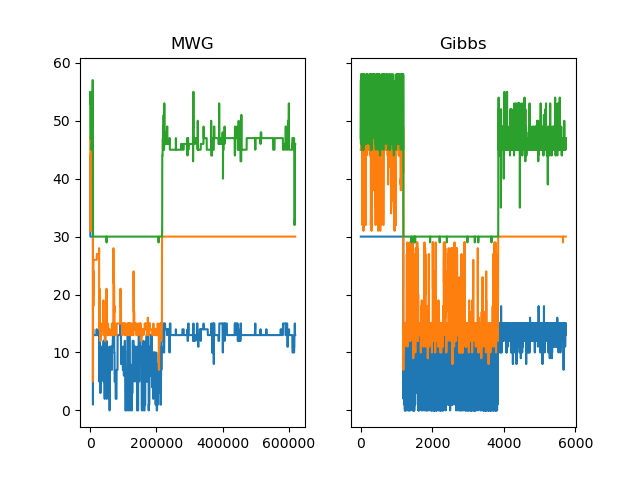
\includegraphics[width=\linewidth]{../../plots/Trace_M4_N60_NMCMC3_seed0_diffind2.png}
        \caption{simulation run \#1}
    \end{subfigure}
    \begin{subfigure}{.3\textwidth}
        \centering
    	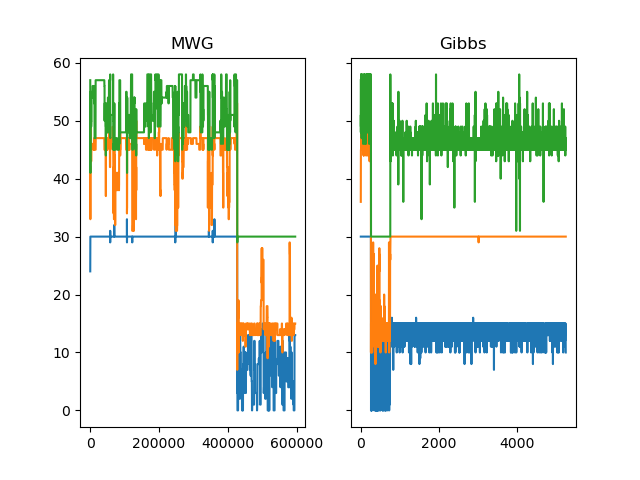
\includegraphics[width=\linewidth]{../../plots/Trace_M4_N60_NMCMC3_seed1_diffind2.png}
    	\caption{simulation run \#2}
	\end{subfigure}
	\begin{subfigure}{.3\textwidth}
	    \centering
    	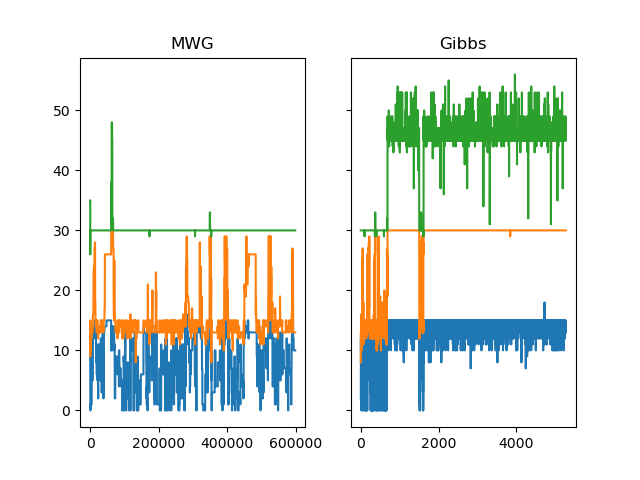
\includegraphics[width=\linewidth]{../../plots/Trace_M4_N60_NMCMC3_seed2_diffind2.png}
    	\label{fig:truth_example}
    	\caption{simulation run \#3}
	\end{subfigure}
	\begin{subfigure}{.3\textwidth}
	    \centering
    	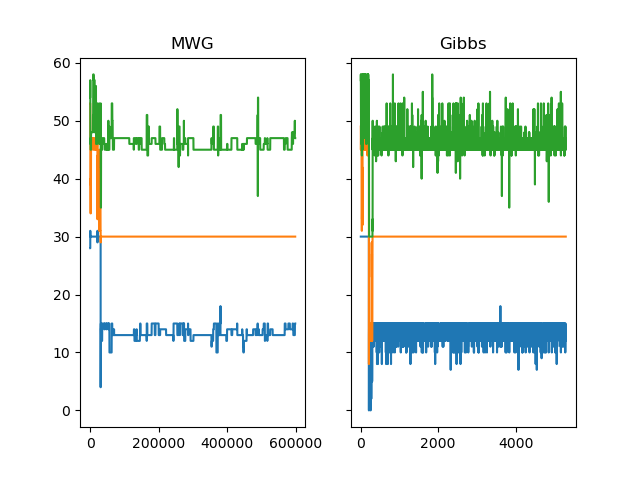
\includegraphics[width=\linewidth]{../../plots/Trace_M4_N60_NMCMC3_seed3_diffind2.png}
    	\caption{simulation run \#4}
	\end{subfigure}
	\begin{subfigure}{.3\textwidth}
	    \centering
    	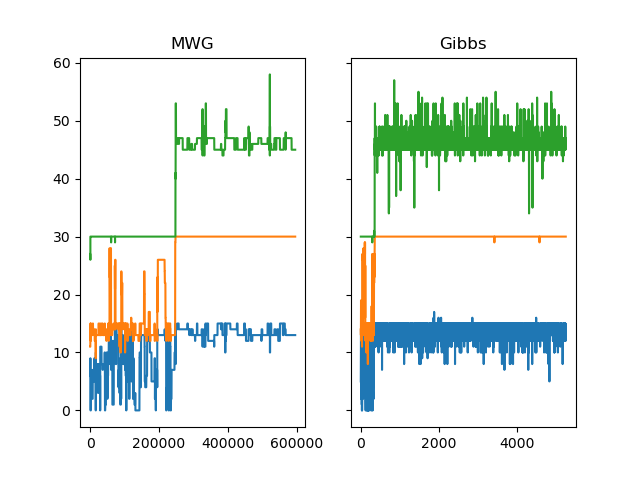
\includegraphics[width=\linewidth]{../../plots/Trace_M4_N60_NMCMC3_seed4_diffind2.png}
		\caption{simulation run \#5}
		\label{fig:eg_before}
	\end{subfigure}
	\caption{Trace plots of entire simulations for the sequence with $n=60, k=3,\bm{\mu} = \{4, 6, 2,4\}, \bm{r} = \{15,30,45\}, T = 32509$.}
\end{figure}

\section{Trace plots after burn in}\label{appendix:trace_burnin}

Each of the five figures below show the trace plots of the change points across the five runs for each sequence. Note that the trace plots exlude samples generated before the corresponding Markov chains have converged. Each color represents a distinct change point. For each plot, the $x$-axis indicate the number of the sample, and the $y$-axis represent the values of each sample (locations of change points).
Empty plots indicate that the simulation has terminated before the Markov chain converged.

\begin{figure}[H]
    \centering
    \begin{subfigure}{.3\textwidth}
    	\centering
        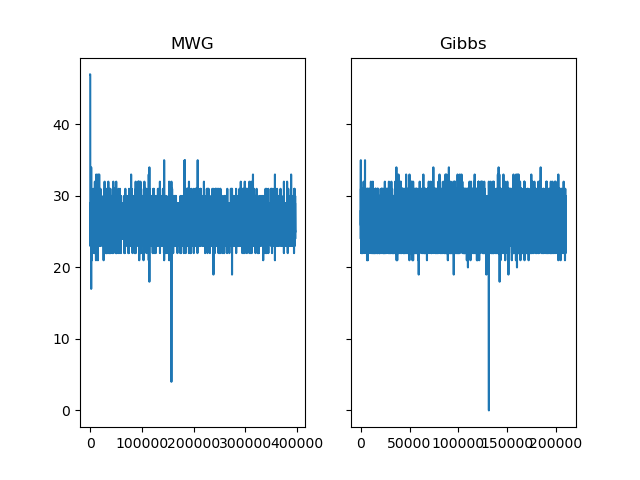
\includegraphics[width=\linewidth]{../../plots/Trace_post_burnin_M2_N50_NMCMC1_seed0_diffind2.png}
        \caption{simulation run \#1}
    \end{subfigure}
    \begin{subfigure}{.3\textwidth}
        \centering
    	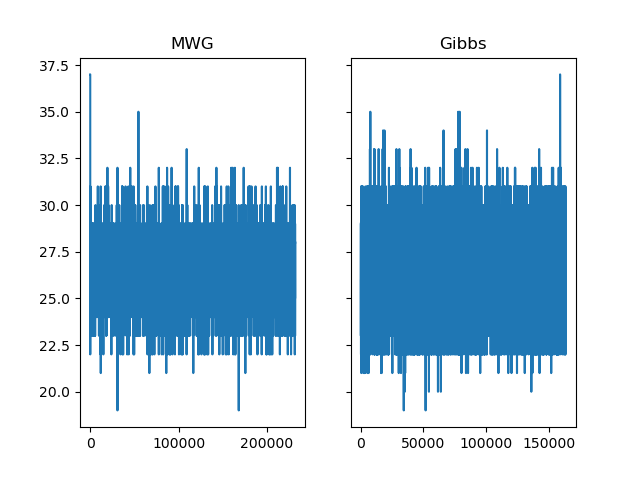
\includegraphics[width=\linewidth]{../../plots/Trace_post_burnin_M2_N50_NMCMC1_seed1_diffind2.png}
    	\caption{simulation run \#2}
	\end{subfigure}
	\begin{subfigure}{.3\textwidth}
	    \centering
    	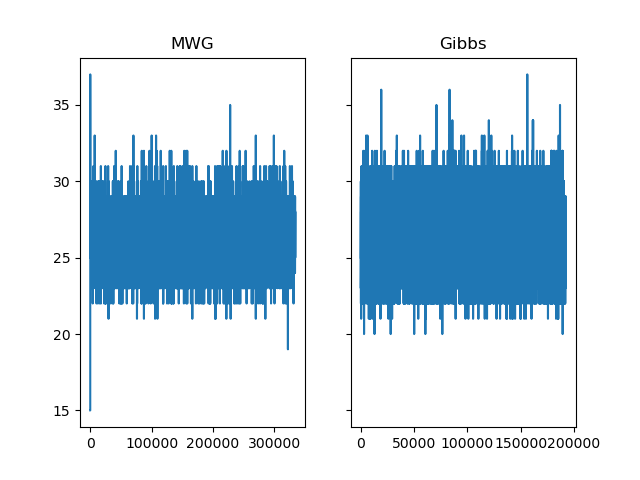
\includegraphics[width=\linewidth]{../../plots/Trace_post_burnin_M2_N50_NMCMC1_seed2_diffind2.png}
    	\caption{simulation run \#3}
	\end{subfigure}
	\begin{subfigure}{.3\textwidth}
	    \centering
    	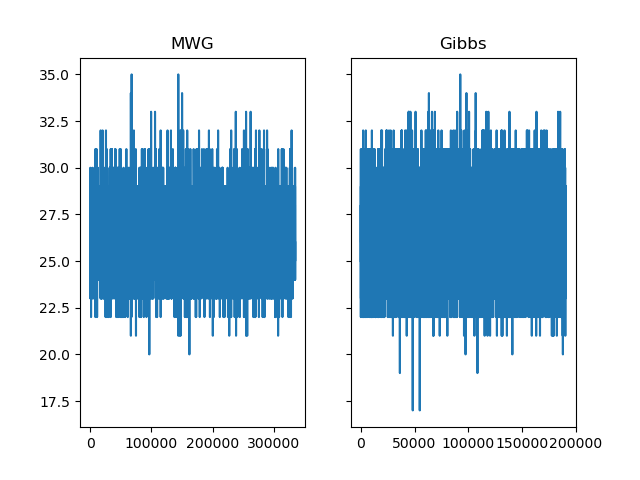
\includegraphics[width=\linewidth]{../../plots/Trace_post_burnin_M2_N50_NMCMC1_seed3_diffind2.png}
    	\caption{simulation run \#4}
	\end{subfigure}
	\begin{subfigure}{.3\textwidth}
	    \centering
    	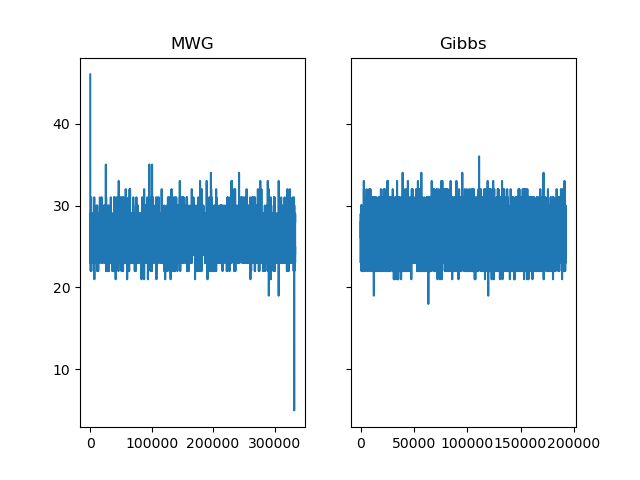
\includegraphics[width=\linewidth]{../../plots/Trace_post_burnin_M2_N50_NMCMC1_seed4_diffind2.png}
    	\caption{simulation run \#5}
	\end{subfigure}
	\caption{Trace plots post burn-in for the sequence with $n=50, k=1, \bm{\mu} = \{2,4\},\bm{r} = \{25\}, T=49$.}
\end{figure}

\begin{figure}[H]
    \centering
    \begin{subfigure}{.3\textwidth}
    	\centering
        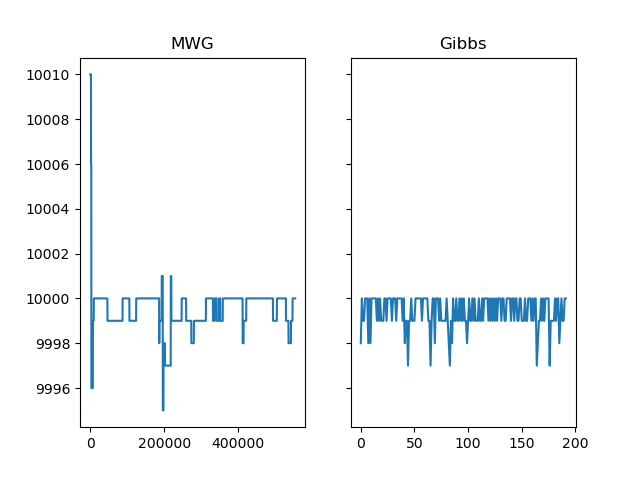
\includegraphics[width=\linewidth]{../../plots/Trace_post_burnin_M2_N20000_NMCMC3_seed0_diffind2.png}
        \caption{simulation run \#1}
    \end{subfigure}
    \begin{subfigure}{.3\textwidth}
        \centering
    	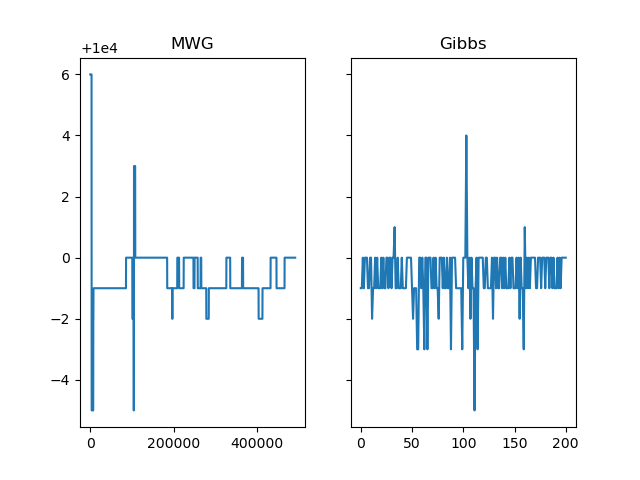
\includegraphics[width=\linewidth]{../../plots/Trace_post_burnin_M2_N20000_NMCMC3_seed1_diffind2.png}
    	\caption{simulation run \#2}
	\end{subfigure}
	\begin{subfigure}{.3\textwidth}
	    \centering
    	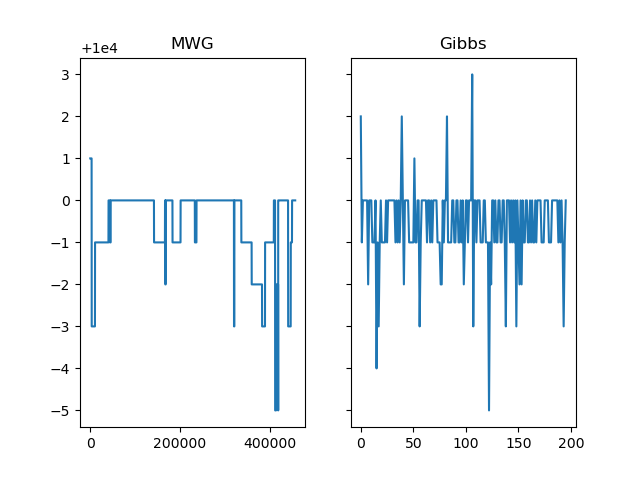
\includegraphics[width=\linewidth]{../../plots/Trace_post_burnin_M2_N20000_NMCMC3_seed2_diffind2.png}
    	\caption{simulation run \#3}
	\end{subfigure}
	\begin{subfigure}{.3\textwidth}
	    \centering
    	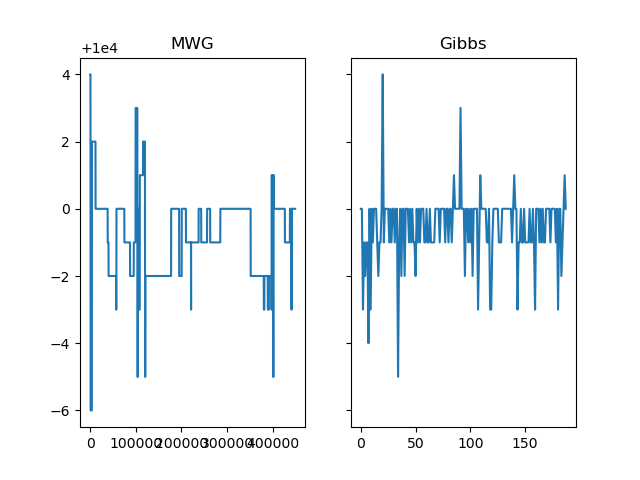
\includegraphics[width=\linewidth]{../../plots/Trace_post_burnin_M2_N20000_NMCMC3_seed3_diffind2.png}
    	\caption{simulation run \#4}
	\end{subfigure}
	\begin{subfigure}{.3\textwidth}
	    \centering
    	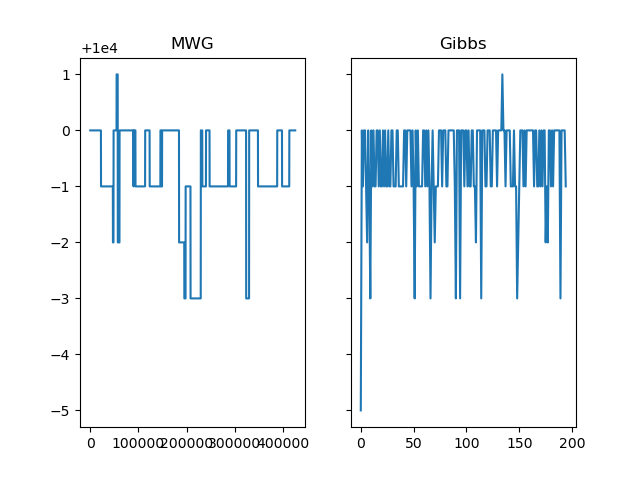
\includegraphics[width=\linewidth]{../../plots/Trace_post_burnin_M2_N20000_NMCMC3_seed4_diffind2.png}
    	\caption{simulation run \#5}
	\end{subfigure}
	\caption{Trace plots post burn-in for the sequence with $n=20000, k=1, \bm{\mu} = \{2,4\}, \bm{r} = \{10000\}, T=19999$.}
\end{figure}

\begin{figure}[H]
    \centering
    \begin{subfigure}{.3\textwidth}
    	\centering
        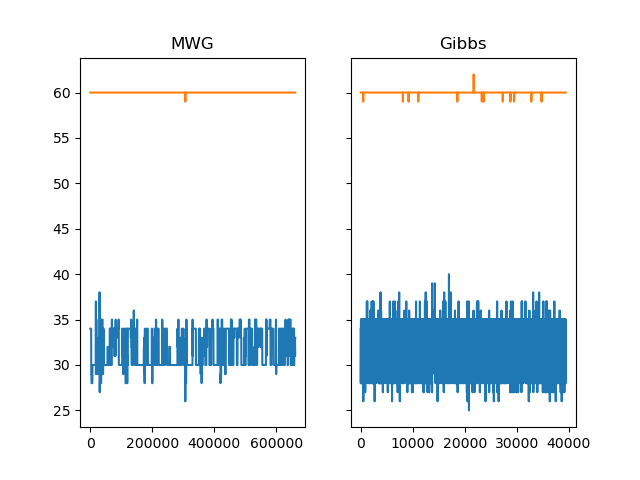
\includegraphics[width=\linewidth]{../../plots/Trace_post_burnin_M3_N100_NMCMC3_seed0_diffind2.png}
        \caption{simulation run \#1}
    \end{subfigure}
    \begin{subfigure}{.3\textwidth}
        \centering
    	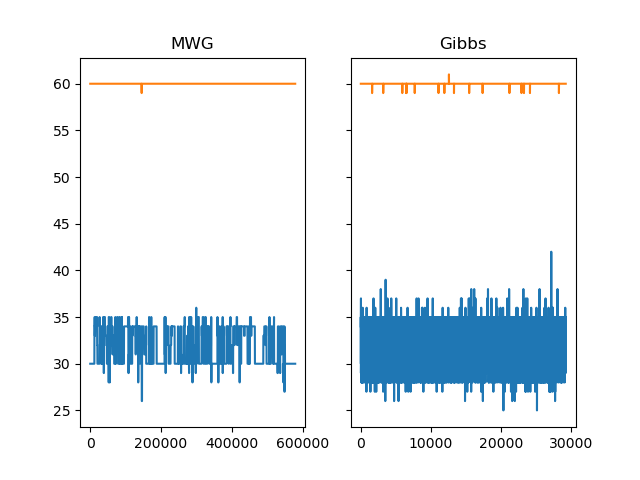
\includegraphics[width=\linewidth]{../../plots/Trace_post_burnin_M3_N100_NMCMC3_seed1_diffind2.png}
    	\caption{simulation run \#2}
	\end{subfigure}
	\begin{subfigure}{.3\textwidth}
	    \centering
    	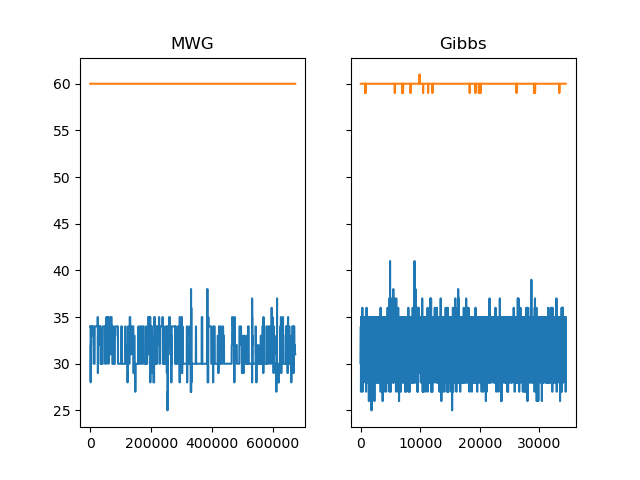
\includegraphics[width=\linewidth]{../../plots/Trace_post_burnin_M3_N100_NMCMC3_seed2_diffind2.png}
    	\caption{simulation run \#3}
	\end{subfigure}
	\begin{subfigure}{.3\textwidth}
	    \centering
    	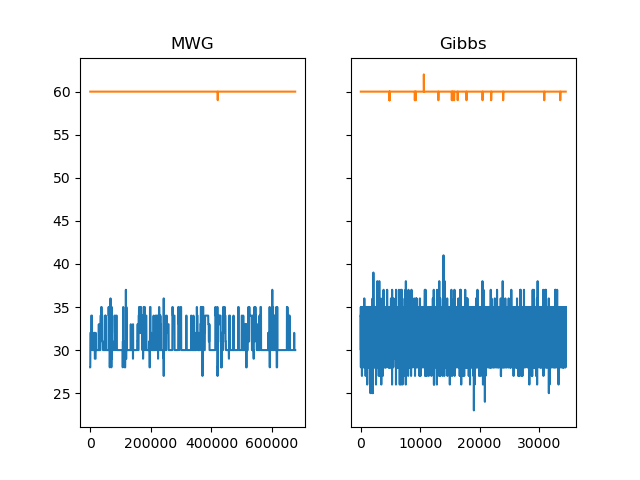
\includegraphics[width=\linewidth]{../../plots/Trace_post_burnin_M3_N100_NMCMC3_seed3_diffind2.png}
    	\caption{simulation run \#4}
	\end{subfigure}
	\begin{subfigure}{.3\textwidth}
	    \centering
    	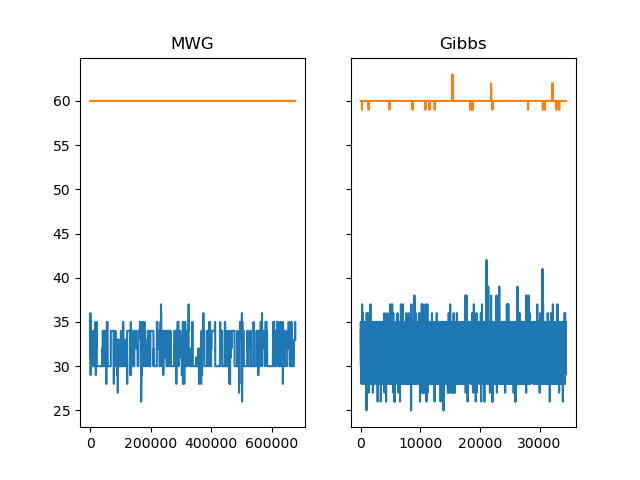
\includegraphics[width=\linewidth]{../../plots/Trace_post_burnin_M3_N100_NMCMC3_seed4_diffind2.png}
    	\caption{simulation run \#5}
	\end{subfigure}
	\caption{Trace plots post burn-in for the sequence with $n=100, k=2, \bm{\mu} = \{4,6,2\}, \bm{r} = \{30,60\}, T=4851$.}
\end{figure}

\begin{figure}[H]
    \centering
    \begin{subfigure}{.3\textwidth}
    	\centering
        \includegraphics[width=\linewidth]{../../plots/Trace_post_burnin_M4_N100_NMCMC3_seed0_diffind2.png}
        \caption{simulation run \#1}
    \end{subfigure}
    \begin{subfigure}{.3\textwidth}
        \centering
    	\includegraphics[width=\linewidth]{../../plots/Trace_post_burnin_M4_N100_NMCMC3_seed1_diffind2.png}
    	\caption{simulation run \#2}
	\end{subfigure}
	\begin{subfigure}{.3\textwidth}
	    \centering
    	\includegraphics[width=\linewidth]{../../plots/Trace_post_burnin_M4_N100_NMCMC3_seed2_diffind2.png}
    	\caption{simulation run \#3}
	\end{subfigure}
	\begin{subfigure}{.3\textwidth}
	    \centering
    	\includegraphics[width=\linewidth]{../../plots/Trace_post_burnin_M4_N100_NMCMC3_seed3_diffind2.png}
    	\caption{simulation run \#4}
	\end{subfigure}
	\begin{subfigure}{.3\textwidth}
	    \centering
    	\includegraphics[width=\linewidth]{../../plots/Trace_post_burnin_M4_N100_NMCMC3_seed4_diffind2.png}
    	\caption{simulation run \#5}
	\end{subfigure}
	\caption{Trace plots post burn-in for the sequence with $n=100, k=3, \bm{\mu} = \{4,6,2,4\}, \bm{r} = \{25,50,75\}, T=156849$.}
\end{figure}

\begin{figure}[H]
    \centering
    \begin{subfigure}{.3\textwidth}
    	\centering
        \includegraphics[width=\linewidth]{../../plots/Trace_post_burnin_M4_N60_NMCMC3_seed0_diffind2.png}
        \caption{simulation run \#1}
    \end{subfigure}
    \begin{subfigure}{.3\textwidth}
        \centering
    	\includegraphics[width=\linewidth]{../../plots/Trace_post_burnin_M4_N60_NMCMC3_seed1_diffind2.png}
    	\caption{simulation run \#2}
	\end{subfigure}
	\begin{subfigure}{.3\textwidth}
	    \centering
    	\includegraphics[width=\linewidth]{../../plots/Trace_post_burnin_M4_N60_NMCMC3_seed2_diffind2.png}
    	\caption{simulation run \#3}
	\end{subfigure}
	\begin{subfigure}{.3\textwidth}
	    \centering
    	\includegraphics[width=\linewidth]{../../plots/Trace_post_burnin_M4_N60_NMCMC3_seed3_diffind2.png}
    	\caption{simulation run \#4}
	\end{subfigure}
	\begin{subfigure}{.3\textwidth}
	    \centering
    	\includegraphics[width=\linewidth]{../../plots/Trace_post_burnin_M4_N60_NMCMC3_seed4_diffind2.png}
    	\caption{simulation run \#5}
    	\label{fig:eg_after}
	\end{subfigure}
	\caption{Trace plots post burn-in for the sequence with $n=60, k=3, \bm{\mu} = \{4,6,2,4\}, \bm{r} = \{15,30,45\}, T=32509$.}
\end{figure}

\section{Wasserstein distance}

\begin{figure}[h]
    \centering
    \begin{subfigure}{0.3\linewidth}
    	\centering
        \includegraphics[width=\linewidth]{../../plots/KL_M2_N50_NMCMC1_seed0_diffind2.png}
    \end{subfigure}
    \begin{subfigure}{0.3\linewidth}
        \centering
    	\includegraphics[width=\linewidth]{../../plots/KL_M2_N20000_NMCMC3_seed0_diffind2.png}
	\end{subfigure}
	\begin{subfigure}{0.3\linewidth}
	    \centering
    	\includegraphics[width=\linewidth]{../../plots/KL_M3_N100_NMCMC3_seed0_diffind2.png}
	\end{subfigure}
	\begin{subfigure}{0.3\linewidth}
	    \centering
    	\includegraphics[width=\linewidth]{../../plots/KL_M4_N100_NMCMC3_seed0_diffind2.png}
	\end{subfigure}
	\begin{subfigure}{0.3\linewidth}
	    \centering
    	\includegraphics[width=\linewidth]{../../plots/KL_M4_N60_NMCMC3_seed0_diffind2.png}
	\end{subfigure}
	\caption{wasserstein}
\end{figure}

\section{Posterior approximation}

\begin{figure}[H]
    \centering
    \begin{subfigure}{.3\textwidth}
    	\centering
        \includegraphics[width=\linewidth]{../../plots/Posterior_post_burnin_M2_N50_NMCMC1_seed0_diffind2.png}
        \caption{simulation run \#1}
    \end{subfigure}
    \begin{subfigure}{.3\textwidth}
        \centering
    	\includegraphics[width=\linewidth]{../../plots/Posterior_post_burnin_M2_N50_NMCMC1_seed1_diffind2.png}
    	\caption{simulation run \#2}
	\end{subfigure}
	\begin{subfigure}{.3\textwidth}
	    \centering
    	\includegraphics[width=\linewidth]{../../plots/Posterior_post_burnin_M2_N50_NMCMC1_seed2_diffind2.png}
    	\caption{simulation run \#3}
	\end{subfigure}
	\begin{subfigure}{.3\textwidth}
	    \centering
    	\includegraphics[width=\linewidth]{../../plots/Posterior_post_burnin_M2_N50_NMCMC1_seed3_diffind2.png}
    	\caption{simulation run \#4}
	\end{subfigure}
	\begin{subfigure}{.3\textwidth}
	    \centering
    	\includegraphics[width=\linewidth]{../../plots/Posterior_post_burnin_M2_N50_NMCMC1_seed4_diffind2.png}
    	\caption{simulation run \#5}
	\end{subfigure}
	\caption{model1: posterior approximation}
\end{figure}

\begin{figure}[H]
    \centering
    \begin{subfigure}{.3\textwidth}
    	\centering
        \includegraphics[width=\linewidth]{../../plots/Posterior_post_burnin_M2_N20000_NMCMC3_seed0_diffind2.png}
        \caption{simulation run \#1}
    \end{subfigure}
    \begin{subfigure}{.3\textwidth}
        \centering
    	\includegraphics[width=\linewidth]{../../plots/Posterior_post_burnin_M2_N20000_NMCMC3_seed1_diffind2.png}
    	\caption{simulation run \#2}
	\end{subfigure}
	\begin{subfigure}{.3\textwidth}
	    \centering
    	\includegraphics[width=\linewidth]{../../plots/Posterior_post_burnin_M2_N20000_NMCMC3_seed2_diffind2.png}
    	\caption{simulation run \#3}
	\end{subfigure}
	\begin{subfigure}{.3\textwidth}
	    \centering
    	\includegraphics[width=\linewidth]{../../plots/Posterior_post_burnin_M2_N20000_NMCMC3_seed3_diffind2.png}
    	\caption{simulation run \#4}
	\end{subfigure}
	\begin{subfigure}{.3\textwidth}
	    \centering
    	\includegraphics[width=\linewidth]{../../plots/Posterior_post_burnin_M2_N20000_NMCMC3_seed4_diffind2.png}
    	\caption{simulation run \#5}
	\end{subfigure}
	\caption{model2: posterior approximation}
\end{figure}

\begin{figure}[H]
    \centering
    \begin{subfigure}{.3\textwidth}
    	\centering
        \includegraphics[width=\linewidth]{../../plots/Posterior_post_burnin_M3_N100_NMCMC3_seed0_diffind2.png}
        \caption{simulation run \#1}
    \end{subfigure}
    \begin{subfigure}{.3\textwidth}
        \centering
    	\includegraphics[width=\linewidth]{../../plots/Posterior_post_burnin_M3_N100_NMCMC3_seed1_diffind2.png}
    	\caption{simulation run \#2}
	\end{subfigure}
	\begin{subfigure}{.3\textwidth}
	    \centering
    	\includegraphics[width=\linewidth]{../../plots/Posterior_post_burnin_M3_N100_NMCMC3_seed2_diffind2.png}
    	\caption{simulation run \#3}
	\end{subfigure}
	\begin{subfigure}{.3\textwidth}
	    \centering
    	\includegraphics[width=\linewidth]{../../plots/Posterior_post_burnin_M3_N100_NMCMC3_seed3_diffind2.png}
    	\caption{simulation run \#4}
	\end{subfigure}
	\begin{subfigure}{.3\textwidth}
	    \centering
    	\includegraphics[width=\linewidth]{../../plots/Posterior_post_burnin_M3_N100_NMCMC3_seed4_diffind2.png}
    	\caption{simulation run \#5}
	\end{subfigure}
	\caption{model3: posterior approximation}
\end{figure}

\begin{figure}[H]
    \centering
    \begin{subfigure}{.3\textwidth}
    	\centering
        \includegraphics[width=\linewidth]{../../plots/Posterior_post_burnin_M4_N100_NMCMC3_seed0_diffind2.png}
        \caption{simulation run \#1}
    \end{subfigure}
    \begin{subfigure}{.3\textwidth}
        \centering
    	\includegraphics[width=\linewidth]{../../plots/Posterior_post_burnin_M4_N100_NMCMC3_seed1_diffind2.png}
    	\caption{simulation run \#2}
	\end{subfigure}
	\begin{subfigure}{.3\textwidth}
	    \centering
    	\includegraphics[width=\linewidth]{../../plots/Posterior_post_burnin_M4_N100_NMCMC3_seed2_diffind2.png}
    	\caption{simulation run \#3}
	\end{subfigure}
	\begin{subfigure}{.3\textwidth}
	    \centering
    	\includegraphics[width=\linewidth]{../../plots/Posterior_post_burnin_M4_N100_NMCMC3_seed3_diffind2.png}
    	\caption{simulation run \#4}
	\end{subfigure}
	\begin{subfigure}{.3\textwidth}
	    \centering
    	\includegraphics[width=\linewidth]{../../plots/Posterior_post_burnin_M4_N100_NMCMC3_seed4_diffind2.png}
    	\caption{simulation run \#5}
	\end{subfigure}
	\caption{model4: posterior approximation}
\end{figure}

\begin{figure}[H]
    \centering
    \begin{subfigure}{.3\textwidth}
    	\centering
        \includegraphics[width=\linewidth]{../../plots/Posterior_post_burnin_M4_N60_NMCMC3_seed0_diffind2.png}
        \caption{simulation run \#1}
    \end{subfigure}
    \begin{subfigure}{.3\textwidth}
        \centering
    	\includegraphics[width=\linewidth]{../../plots/Posterior_post_burnin_M4_N60_NMCMC3_seed1_diffind2.png}
    	\caption{simulation run \#2}
	\end{subfigure}
	\begin{subfigure}{.3\textwidth}
	    \centering
    	\includegraphics[width=\linewidth]{../../plots/Posterior_post_burnin_M4_N60_NMCMC3_seed2_diffind2.png}
    	\caption{simulation run \#3}
	\end{subfigure}
	\begin{subfigure}{.3\textwidth}
	    \centering
    	\includegraphics[width=\linewidth]{../../plots/Posterior_post_burnin_M4_N60_NMCMC3_seed3_diffind2.png}
    	\caption{simulation run \#4}
	\end{subfigure}
	\begin{subfigure}{.3\textwidth}
	    \centering
    	\includegraphics[width=\linewidth]{../../plots/Posterior_post_burnin_M4_N60_NMCMC3_seed4_diffind2.png}
    	\caption{simulation run \#5}
	\end{subfigure}
	\caption{model5: posterior approximation}
\end{figure}

\section{ESS and MCSE}

\begin{figure}[H]
    \centering
    \begin{subfigure}{.3\textwidth}
    	\centering
        \includegraphics[width=\linewidth]{../../plots/ess_se_M2_N50_NMCMC1_seed0_diffind2.png}
    \end{subfigure}
    \begin{subfigure}{.3\textwidth}
        \centering
    	\includegraphics[width=\linewidth]{../../plots/ess_se_M2_N20000_NMCMC3_seed0_diffind2.png}
	\end{subfigure}
	\begin{subfigure}{.3\textwidth}
	    \centering
    	\includegraphics[width=\linewidth]{../../plots/ess_se_M3_N100_NMCMC3_seed0_diffind2.png}
	\end{subfigure}
	\begin{subfigure}{.3\textwidth}
	    \centering
    	\includegraphics[width=\linewidth]{../../plots/ess_se_M4_N100_NMCMC3_seed0_diffind2.png}
	\end{subfigure}
	\begin{subfigure}{.3\textwidth}
	    \centering
    	\includegraphics[width=\linewidth]{../../plots/ess_se_M4_N60_NMCMC3_seed0_diffind2.png}
	\end{subfigure}
	\caption{ess and se}
\end{figure}